\chapter{Introduction}
\label{ch:introduction}
The use of scientific computing to studying the Qur'\=an is still in its early stage in the fields of Islamic Studies and Statistical and Machine Learning applications. This is evident from the fact that there is no known books yet on this topic as far as the knowledge of the author at the time of writing. In addition to this, because this paper tackles methodology from both fields, it therefore benefit not only the researchers from Islamic Studies but also Statisticians and Machine Learning practitioners who are into text analytics. Having said that, it is necessary to provide context to audiences of these disciplines on both backgrounds on the state of Qur'\=anic studies and the increasing adoption of scientific methodologies to studying humanities.
\section{Background}
The Qur'\=an or \arb[trans]{al-qur'An} \arb{al-qur'An} meaning \textit{the recitation}, the holy book of Islam, is revered by 1.9 billion (according to 2020 projection of \shortciteA[p.~13]{pewresearch}) Muslims across the globe as the literal words of God. Muslims believed that the Qur'\=an was gradually revealed (Qur'\=an 25:32) to Prophet Muhammad \arb{\arbmark{slm}} through angel \arb[trans]{jibrIl} \arb{jibrIl} or Gabriel (Qur'\=an 2:97). The Qur'\=an contains 77,429 Arabic words in total, which covers only 56 percent of the Greek New Testament which has 138,020 words in total \cite[p.~11]{sinai2017}. 

The Qur'\=an is divided into \arb[trans]{sUwar} \arb{sUwar} (\textit{plural} of \arb[trans]{sUraT} \arb{sUraT}) which are the equivalent of chapters, each containing \arb[trans]{'AyAt} \arb{'AyAt} (\textit{plural} of \arb[trans]{'AyaT} \arb{'AyaT} meaning \textit{signs}), which are the equivalent of verses. The \arb[trans]{sUwar} \arb{sUwar} are not arranged in chronological order as in the Bible's books and chapters, but rather arranged in monotonically decreasing length of number of verses after the first \arb[trans]{sUraT} \arb{sUraT} (\textit{see} Figure \ref{fig:ayah_word_count}). The \arb[trans]{sUwar} \arb{sUwar} of the Qur'\=an can be categorized into two types: the \arb[trans]{makkiyyaT} \arb{makkiyyaT} (Meccan) and \arb[trans]{madaniyyaT} \arb{madaniyyaT} (Medinan). The categories refer to the geographical location of where the \arb[trans]{sUraT} \arb{sUraT} was revealed to Prophet Muhammad \arb{\arbmark{slm}}. Figure \ref{fig:ayah_word_count} shows the groupings of the \arb[trans]{sUwar} \arb{sUwar}. Note that some of the \arb[trans]{sUwar} \arb{sUwar} have mixed geographical locations\footnote{\textit{see} list of the location in \url{https://tanzil.net/docs/revelation_order}}, that is, a few of the \arb[trans]{'AyAt} \arb{'AyAt} in it were revealed in other geographical location apart from the geographical location of the rest of the \arb[trans]{'AyAt} \arb{'AyAt}. Therefore, the categorization in Figure \ref{fig:ayah_word_count} highlights the geographical location of the majority of the \arb[trans]{'AyAt} \arb{'AyAt} in the \arb[trans]{sUraT} \arb{sUraT}.

\begin{figure}[!b]
    \centering
    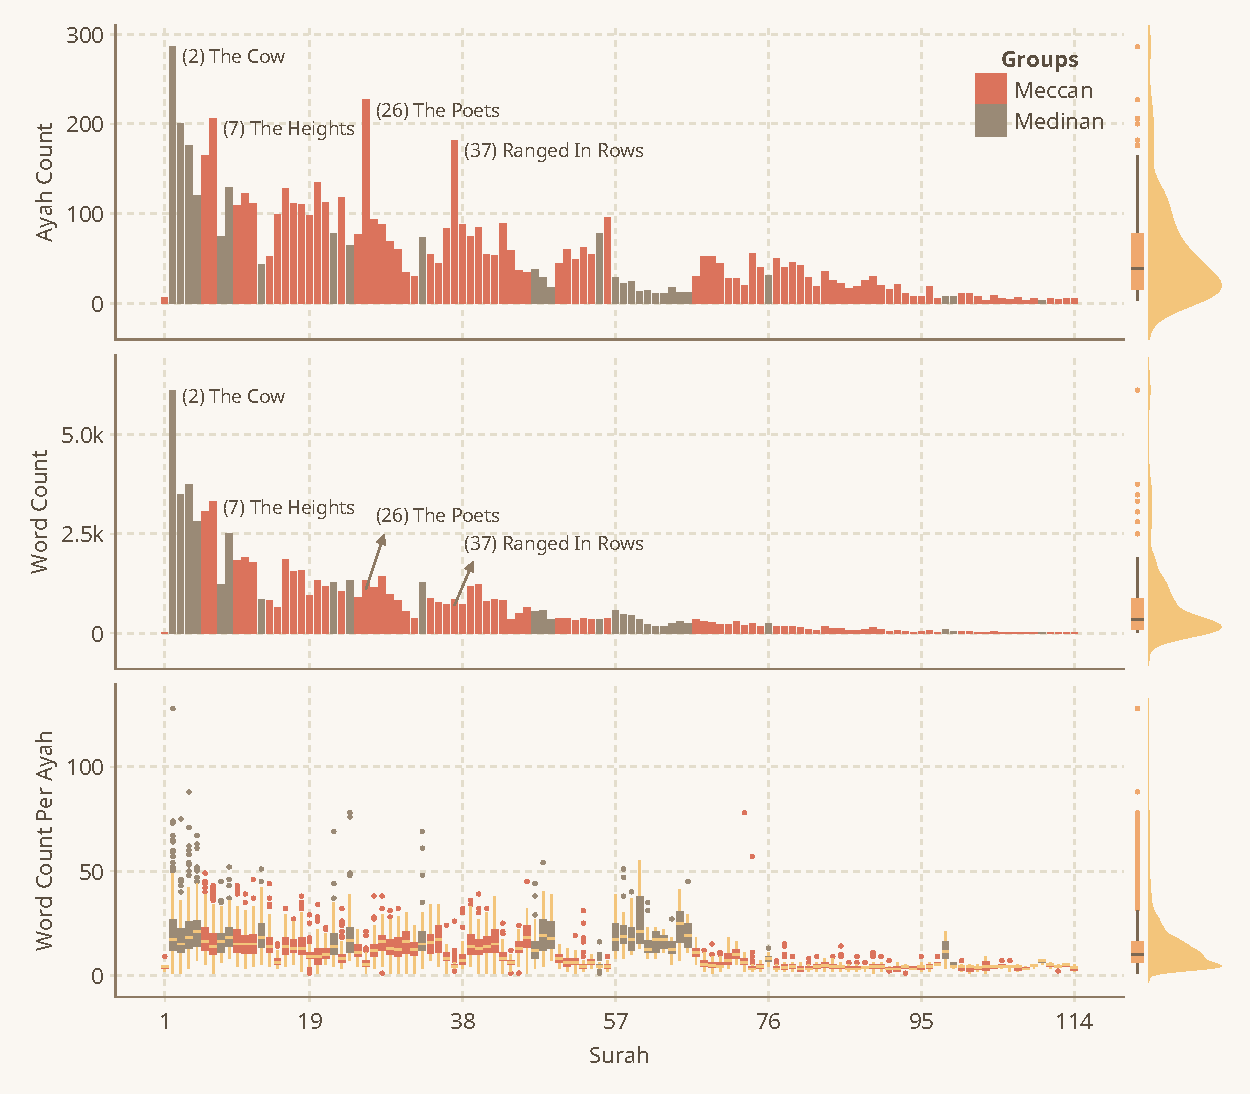
\includegraphics[width=\textwidth]{img/plot1.pdf}
    \caption{Statistics of the words and \arb[trans]{'AyAt} \arb{'AyAt} (verses) of the Qur'\=an}
    \label{fig:ayah_word_count}
\end{figure}

Attempts at understanding the Qur'\=an by Qur'\=anic scholars were mostly done with the use of manual processes, that is, studying the scriptures by going through its content manually line-by-line or one-at-a-time. However, with the advent of computers, some researchers have started using it to aid in their study. The first known to have used computers for studying the Qur'\=an was likely Rashad Khalifa in 1968\footnote{\url{https://www.masjidtucson.org/quran/miracle/a_profound_miracle_sura68nun133.html}}, where he studied the significance of the mysterious initials at the beginning of some \arb[trans]{sUwar} \arb{sUwar}. Rashad uploaded the Qur'\=an into his computer by transliterating the Arabic letters and other Qur'\=anic orthographies into Roman letters and symbols that the computer can easily parse. This approach of using computers to find new insights is more common in the field of science, and it was new to the field of Qur'\=anic studies.

Indeed, to proceed with the use of scientific computing, the Qur'\=an will be treated as the data that needs to be analyzed using a scientific process called Natural Language Processing (NLP), a branch of Machine Learning (ML) that aims to understand natural languages, such as Arabic. To instruct the computer to do Statistical analyses or ML, one needs to use a \textit{software application} or a formal\footnote{"formal" because these languages were invented by man for particular purpose, in this case to communicate with computers} language called \textit{programming language}. There are several programming languages that the computer can understand. The popular one for researchers in the field of sciences are Python \cite{van1995python}, R \cite{rprogramming}, and sometimes Julia \shortcite{Julia2017}. These programming languages will be used to construct instructions for computers. Therefore, if the data is the Qur'\=an, then there should be a way to interface with it using any of these programming languages; or alternatively, there should be a way to upload it into the chosen programming language and encode the Arabic letters into something that can be easily parsed by the computers, like what Rashad \mbox{Khalifa} did. Having said that, there are indeed some programming languages with libraries or packages for interfacing with the Qur'\=an, and this is true for Python, R, and \mbox{Julia}. For this study, the three programming languages will be used. The reason is that the scope and objective of this paper covers a wide range of statistical and Machine Learning methodologies, and that the three programming languages have advantages in certain methods and not on others. As such, the paper will use the appropriate programming language that is more fit for the task. The ruling is that Julia will be used for interfacing with the Qur'\=an texts since its library for it has more features \cite<\textit{see}>{asaad2021qurantree} compared to R and Python. The said Julia library is the QuranTree.jl\footnote{\url{https://alstat.github.io/QuranTree.jl/stable/}}. QuranTree.jl is based on Tanzil\footnote{\url{https://tanzil.net/download/}} for the Qur'\=anic Arabic texts, and \citeA{dukes-habash-2010-morphological} for morphological annotation, which both libraries from R and Python do not have in terms of morphological annotations from \citeA{dukes-habash-2010-morphological}. On the other hand, both R and Python will be used for libraries that are not available in Julia. In particular, R is known for niche statistical libraries since it was made for statistical computation, whereas Python is now popular for Deep Learning frameworks for complex modeling like TensorFlow\footnote{\url{https://www.tensorflow.org/}} (a library made by Google\footnote{\url{https://research.google/}}) and PyTorch\footnote{\url{https://pytorch.org/}} (a library made by Meta\footnote{\url{https://ai.meta.com/}}). 

Given the programming languages, next is to understand how Statistics and Machine Learning can help in studying the Qur'\=an. Statistics is a branch of Science that aims to study features or characteristics of data generated from a random phenomenon. The findings of Statistical analyses can then be used to make decisions, conclusions or predictions of the general population of the data or general characteristics of the data. Machine Learning or ML, on the other hand, is a branch of Artificial Intelligence that heavily intersects with Statistics, albeit with distinct differences as well. Both Statistics and ML aims to characterize data by learning its features, but ML researchers have been aiming on complex models that are often inspired by simpler models from Statistics. Therefore, one can think of Statistics as one of the fundamentals of ML. 

One of the goals of Statistics and Machine Learning is to summarize all of the learned features of the data into a hypothesized equation or hypothesized mathematical formula by optimizing the parameters or weights of this equation or formula to capture \textit{most}\footnote{Not all characteristics of the data can be captured by the model, and those that are not captured are called the errors, and the goal is to minimize the errors into something tolerable.} of the characteristics of the data. The idea stems from the fact that any data point is simply a sum of its components, which are factors known to affect the data point. For example, the volume of orders in a restaurant is dependent on the time of the day. More orders are expected during lunch and dinner. Hence, volume of orders as data points can be derived from the sum of factors such as time of the day, and also day of the week (assuming more orders during weekends or weekdays). Therefore, from this example, any data point is affected by factors that can be translated into math so that their sum results into the data points we want, like the volume of orders. It is for this reason why the hypothesized mathematical equations or formula are used for summarizing the features and capturing the characteristics of data. It is called \textit{hypothesized equation} since the researcher is the one who decide which family of equations best describe the characteristics of the data. There are many possible mathematical formulae that can be constructed, and not all can be used to describe the data, this is why the researcher is the one who decide. So that, those equations that can be used for understanding the data are special enough that they are referred to as \textit{models}. Mathematically and in general, a model can be related to the data as follows:
\begin{equation}\label{eq:general_model}
    y=h(x|\boldsymbol{\theta})+\varepsilon,
\end{equation}
where $h(x|\boldsymbol{\theta})$ is the hypothesized model taking the input data $x$ (from the examples discussed above, these are the values of the factors affecting in the volume of orders), where $x\in\mathscr{X}$ (from the examples discussed above, $\mathscr{X}$ is the set containing all values of the factors mentioned), and outputs a target data $y$ (from the examples discussed above, this is the volume of orders), where $y\in\mathscr{Y}$. Therefore, $h:\mathscr{X}\rightarrow\mathscr{Y}$, meaning $h$ maps the factors or features into the set of the target variable $y$. The $\varepsilon$ is the error that the hypothesized model $h(x|\boldsymbol{\theta})$ cannot capture even after finding the best configuration of its parameter $\boldsymbol{\theta}$. Ideally the error or \textit{residual} or sometimes called \textit{innovation}, $\varepsilon$, should exhibit a \textit{random noise} for us to say that the hypothetical model $h(x|\boldsymbol{\theta})$ has captured well the core characteristics of the data $(x,y)$. These random noise are data points that could have come from other factors that are not available in the given data, $(x,y)$. Therefore, the idea of modeling is to find the optimal value of $\boldsymbol{\theta}$ such that the error  between the actual data (represented by $y$ below) and the predicted one $\hat{y}$, is as small as as possible or tolerable:
\begin{equation}
    \varepsilon:=y-\hat{y}=y-h(x|\boldsymbol{\theta}).
\end{equation}

To help understand the concept of modeling, and relate it to the fashion industry, which the author assumes most readers are familiar with, a model in a fashion industry is responsible for representing the characteristics of the target customers (in Eq. \ref{eq:general_model} this is $y$). Therefore, for a clothing company, they hire Asian models (in Eq. \ref{eq:general_model}, this is $h(x|\boldsymbol{\theta})$) to target Asian customers (in Eq. \ref{eq:general_model} this is $y$). So that, when these models wore the clothes sold by the said company, the potential customer will more or less be able to relate to the model, and be able to imagine themselves wearing that same clothes as well, which help them incline to buying the said clothing. The model, therefore, does not necessarily have the looks of every target Asian customers, but at least in terms of height, skin tone, hair, and other common Asian features, the model will likely have it, or at least the difference is more or less minimal (in Eq. \ref{eq:general_model}, the difference is represented by $\varepsilon:=y-\hat{y}$). The question now is, what are the benefits that this model can bring to the clothing company? Well, the clothing company will be able to create products that are tailored to their Asian customers using the said model, since the company will have the right baseline measurements needed. Relating this analogy to the technical concept discussed earlier, you can think of the target customers as the
real or actual data (in Eq. \ref{eq:general_model} this is $y$), and the model as the same technical term use in Machine Learning and Statistics (in Eq. \ref{eq:general_model} this is $h(x|\boldsymbol{\theta})$), but this time this technical model is expected to capture the characteristics of the real data analogous to fashion model that is expected to capture the characteristics of the target customer. This Statistical or Machine Learning model brings the following benefits: researchers will be able to study the real data by simply using the model to answer questions that are not available in the sampled real data.

\section{Rationale of the Study}\label{sec:rationale}
Having understood the background of this study, let's turn our attention to the rationale. When it comes to modeling the characteristics of any data, there are several ways to do it, and it all depends on the questions one would like to answer. Apart from this, it also depends on the richness of the data. This is true for the Qur'\=an. The rich morphological annotations done by \citeA{dukes-habash-2010-morphological} has opened a lot of opportunities for statistical analyses. It is even hard to decide on where to start since this morphological data has not been extensively studied yet, at least based from the survey of \shortciteA{DarwishHabash2021} and \shortciteA{bashir2023arabic}, and apart from the work of  \shortciteA{dukes2013supervised} and \shortciteA{dukes2010online} on the dependency graph of the morphological annotations of their original work \cite{dukes-habash-2010-morphological}. Most of the natural language processing studies done on the Qur'\=an have revolved around corpus creation on annotations of mophological features of the Qur'\=an \shortcite{dukes-habash-2010-morphological}, Qur'\=an's pronouns annotations \shortcite{sharaf2012}, the \arb[trans]{'AyAt} \arb{'AyAt} similarity annotations \shortcite{sharaf2012b}, and comparative analyses of corpora \shortcite{sabtan2017morphological}; Qur'\=an's stemming system \shortcite{thabet2004} and its tokenization\footnote{\textit{See} Section \ref{sec:text_tokenization}} \shortcite{thabet2005}; thematic clustering\footnote{\textit{See} Section \ref{sec:thematic-analyses}} of some \arb[trans]{sUwar} \arb{sUwar} \shortcite{siddiqui2013, alhawarat2015extracting}; semantic techologies for improved keyword search in the Qur'\=an \shortcite{afzal2019semantically}, and criterias for evaluating the search algorithms \shortcite{alqahtani2017evaluation}; Qur'\=an's recitation validation through speech recognition \shortcite{ahsiahNoor2013, abroNaqvi2012,ahmed2017verification}; Qur'\=an's authorship analyses in comparison to Prophet Muhammad's \arb{\arbmark{slm}} sayings or statements; Qur'\=an's grammatical analyses by predicting the parts-of-speech (POS) \shortcite{ELAFFENDI202135}, \arb[trans]{'i`rAb} \arb{'i`rAb}\footnote{Refers to the inflectional system used to indicate the grammatical case, mood, and other syntactical features of words, particularly nouns, pronouns, adjectives, and verbs.} modeling through enhanced context-free grammar \shortcite{MANNAA20228909}; Word embedding\footnote{\textit{See} Section \ref{sec:word-embeddings}} models for the Qur'\=an, such as the use of doc2vec based vectorization of the \arb[trans]{'AyAt} \arb{'AyAt} \shortcite{ALSHAMMERI2021351}, and other word embedding methods trained on different Islamic texts like \arb[trans]{'a.hAdI_t} \arb{'a.hAdI_t}\footnote{Plural of \arb[trans]{hadI_t} \arb{hadI_t}, which means the recorded words and practices of Prophet Muhammad \arb{\arbmark{slm}}} \shortcite{aliMaged2020}, and the use of Bidirectional Encoding Representation from Transformers\footnote{\textit{See} Section \ref{sec:bert}} (BERT) like CL-AraBERT \shortcite{MALHAS2022103068}; and Qur'\=an's text classification of \arb[trans]{'AyAt} \arb{'AyAt} into their corresponding \arb[trans]{sUraT} \arb{sUraT} \shortcite{al2005statistical}, and into their place of revelation \shortcite{nassourou2011}.

Among the studies mentioned above on the application of Natural Language Processing to the Qur'\=an, including those surveyed by \shortciteA{DarwishHabash2021} and \shortciteA{bashir2023arabic}, none has looked into the statistical analyses of the \textit{rhythmic patterns} of the Qur'\=an. This is the most prevalent feature of the Qur'\=an, in that it rhymes from the very first chapter all the way to the last. This unique characteristics can be easily confirmed by simply searching on YouTube\footnote{\url{https://www.youtube.com/}} for Qur'anic recitation of say \arb[trans]{sUraTu 'l-baqaraT} \arb{sUraTu 'l-baqaraT}, the second chapter of the Qur'an. This unique characteristics separates this book to the rest, and more on this on Chapter \ref{ch:quran_history} of this paper, but this obvious feature of the Qur'an has never been analyzed statistically. This is the first paper to the best knowledge of the author to do so. 

Further, none has looked into the \textit{concentrism theory} yet as posited by \shortcite{farrin2014structure}. The said author proposed that the Qur'\=an follows such structural characteristics. This is indeed a challenge to do computationally since there is no known statistical or mathematical theory that already accommodates this, one needs to create a formal mathematical definitions and theories to do so. This is also the first paper to investigate this from mathematical and statistical point of views to the best knowledge of the author. Moreover, the emergence of Retrieval-Augmented Generation was only applied so far for Arabic language \shortcite{Abdelazim2023, mahboub2024evaluation} but no specific study yet for the use of it as a tool for Qur'\=anic study. Hence, this new way of retrieving information through Large Language Models (LLMs) proposed in this paper for the Qur'\=an will likely be among the pioneers as well. Finally, the statistical analyses of the morphological features of the Qur'\=an from the work of \shortciteA{dukes-habash-2010-morphological}, particularly on the parts-of-speech and name entities, will like be pioneered by this paper as well. Having said these, the following section will discuss the objectives of this paper.

\section{Objectives}\label{sec:objectives}
The following are the general and specific objectives of this paper:
\begin{enumerate}
    \item What are the structural characteristics of the Qur'an that can be extracted from its rich morphologies using statistical and large language models?
    \begin{enumerate}
        \item What are the statistics of the Qur'\=an's morphological features in terms of its parts of speech and selected entities like God's name and the prophets names mentioned?
        
        \item How do the rhythmic signatures of the Qur'\=an of the verses looks like and what are statistical insights that can be extracted?
    \end{enumerate}
    
    \item What other insights that can be extracted from the semantics of the Qur'an's texts using statistical and large language models?
    \begin{enumerate}
        \item How does the theory of \textit{concentrism} be formulated statistically, and what are the insights from the statistical and large language models on this? 
        
        \item How do the \arb[trans]{sUwar} \arb{sUwar} are organized in terms of the topics? What are the themes that can be extracted for each of the surahs?
        
        \item How do these extracted themes compare to the summaries of Abdel\linebreak Haleem's English translation of the Qur'an?
    \end{enumerate}
    
    \item How does these combinations of statistical, machine learning, and artificial intelligence with the Muslim's traditional literatures help in understanding the Qur'\=an, especially with the advent of Generative AI?
\end{enumerate}

\section{Significance of the Study}\label{sec:significance}
While the Qur'\=an has been extensively studied by Muslims and non-Muslims scholars alike, especially in the topic of Meccan and Medinan surahs, there is still a lot to uncover from the perspective of Computational Statistics and AI. More specifically, the significance of this study is that it brings forward new ways of extracting insights from the Qur'\=an by leveraging Computations, Statistics, Machine Learning, and AI, that is still in its early stage in the field of Qur'\=anic Studies. This is especially true for Islamic Studies researcher, which the author hopes to benefit and get interested in Islamicate Digital Humanities, a new field which aims to take advantage of the scientific computations for studying Islamic texts, which the author hopes to have in any Islamic institute. 

Further, since this paper combines the several fields (Islamic Studies, Statistics, and Machine Learning), the results will also contain mathematical theories that is hoped to advance the field of Statistics and Machine Learning as well. With that said, the author would like to also emphasize the opportunities that scientific methodologies can bring to studying Islamic studies, especially for Muslim researchers who are in the field of science. Finally, this new perspective or process of studying the scripture not only aids the scholars of the Islamic Studies, Statistics, and Machine Learning, but may also contribute indirectly to community development and policy makers who use Qur'\=an as part of their decision making.
\section{Scope of the Study}
The paper will cover all chapters of the Qur'\=an as much as possible, except maybe for cases like thematic modeling on very short \arb[trans]{sUwar} \arb{sUwar}, since topics on these \arb[trans]{sUwar} \arb{sUwar} may be obvious already or easier to see due to very short number of \arb[trans]{'ayaT} \arb{'ayaT}. However, for cases where the analyses is not at the level of \arb[trans]{sUraT} \arb{sUraT}, but rather on the level of the Qur'\=an as a whole, then all of the \arb[trans]{sUwar} \arb{sUwar} will be used. 
\section{Thesis Organization}
The paper is organized as follows: Chapter \ref{ch:rrl} will discuss the related literatures; Chapter \ref{ch:tf-cf} will discuss the Theoretical and Conceptual Frameworks; Chapter \ref{ch:quran_history} will discuss the historical background of the Qur'\=an; Chapter \ref{ch:statistics} will discuss the background on Probability and Statistics; Chapter \ref{ch:neural-networks} the backgound on Neural Networks and Transformers, this is the core model used by most AI nowadays which is also part of the models of this paper; Chapter \ref{ch:nlp} will discuss the backgound and concept of Natural Language Processing, that is, how to process the Qur'\=anic texts; Chapter \ref{ch:methodology} will discuss the Methodology of this paper; Chapter \ref{ch:results} will discuss the results of the paper; Chapter \ref{ch:conclusion} will discuss the conclusion and recommendation of the paper.
\section{Mathematical Sections}
Succeeding chapters will have a lot of mathematical formulas, and it is important to have some guide on the flow of presentation. Like any humanities studies, Mathematics is mostly concern with understanding facts about objects that is being studied. For Islamic studies, these objects can be physical like Qur'\=an and other Islamic texts, or metaphysical like understanding the purpose of life. For Mathematics, the objects can be explicit or abstract as well, but it does revolve heavily on numbers and logics, and like other domain it studies facts about these objects. With that said, any object being studied in Mathematics are presented as Definitions, a formal way of defining terms or objects, see for example the following presented in Chapter \ref{ch:statistics}:
\begin{defn}[Mean]\label{defn:mean-1}
Let $x_i, i\in\{1,\cdots,n\}$ where $n\in\mathbb{N}$, then the \textit{mean} of $x_i$s is defined as follows:
\begin{equation}\label{eq:mean-formula-1}
    \bar{x} = \sum_{i=1}^n x_i, \qquad\text{where}\;x_i \in\mathbb{R}.
\end{equation}
\end{defn}
This is a Definition of a mathematical object called \textit{mean} or \textit{average}. It is presented as a section in this paper like the one above, and this is the convention in any advanced mathematical books and courses. In this paper, and for the sake of brevity, when referring to Definition \ref{defn:mean-1}, it will be written as Defn. \ref{defn:mean-1}. Also, instead of writing Equation \ref{eq:mean-formula-1} to refer to the above equation, it will be written as Eq. \ref{eq:mean-formula-1}. Further, using these objects, facts about these them are found through proof using mathematical computations and logics. An example of this is the result or fact about another mathematical object called \textit{Gaussian Process} discussed in Section \ref{sec:bayes-opt} of this paper, see below.
\begin{prop}\label{prop:jointpdf-1}
    From Proposition \ref{prop:hypedist}, suppose $\boldsymbol{\delta}_{*}:=[\gamma(\mathbf{v}_{n+1}),\cdots,\gamma(\mathbf{v}_{n+p})]^{\top}$, such that $\boldsymbol{\delta}_{*}\overset{\mathrm{iid}}{\sim}\mathcal{N}_p(\mathbf{m}_*,\mathbf{K}_*)$ then 
    \begin{equation}
        \left[
        \begin{matrix}
            \boldsymbol{\delta}\\
            \boldsymbol{\delta}_{*}\\
        \end{matrix}
        \right]\overset{\mathrm{iid}}{\sim}
        \mathcal{N}_{n+p}\left(\left[
        \begin{matrix}
            \mathbf{m}\\
            \mathbf{m}_{*}\\
        \end{matrix}
        \right],\left[
        \begin{matrix}
            \mathbf{K}&\mathbf{K}_{*}\\
            \mathbf{K}_{*}^{\top}&\mathbf{K}_{**}\\
        \end{matrix}
        \right]\right)
    \end{equation}
\end{prop}
\begin{proof}
    Let $\mathbf{u}:=[\boldsymbol{\delta},\boldsymbol{\delta}_{*}]^{\top}$, then $\mathbf{u}=[\gamma(\mathbf{v}_1),\cdots,\gamma(\mathbf{v}_{n+p})]^{\top}$. Further, since $\mathbf{\gamma}(\mathbf{v}_i)\overset{\mathrm{iid}}{\sim}\mathcal{N}(m(\mathbf{v}_i),k(\mathbf{v}_i,\mathbf{v}_i)),\forall i\in\mathbb{N}_{\leq n+p}$, then the joint distribution of the $\gamma(\mathbf{v}_i)$s, i.e. $\mathrm{Pr}(\mathbf{u})$, follows from the proof of Theorem 1.2.9 of \citeA{muirhead2005}.
\end{proof}
Verified facts that are of significant findings are sectioned as Theorem in mathematics, whereas those that are proposed are called Proposition. Other small results or facts supporting the Proposition are sectioned as Corollary. There are other sections in mathematics for formal presentation of facts and results, but those are the ones used in this paper. These sections are present in most chapters of this paper especially those dealing with math, and this brief guide hopes to help Islamic students or reseachers navigate the paper.